\documentclass[10pt,handout]{beamer}\usepackage[]{graphicx}\usepackage[]{color}
% maxwidth is the original width if it is less than linewidth
% otherwise use linewidth (to make sure the graphics do not exceed the margin)
\makeatletter
\def\maxwidth{ %
  \ifdim\Gin@nat@width>\linewidth
    \linewidth
  \else
    \Gin@nat@width
  \fi
}
\makeatother

\definecolor{fgcolor}{rgb}{0.345, 0.345, 0.345}
\newcommand{\hlnum}[1]{\textcolor[rgb]{0.686,0.059,0.569}{#1}}%
\newcommand{\hlstr}[1]{\textcolor[rgb]{0.192,0.494,0.8}{#1}}%
\newcommand{\hlcom}[1]{\textcolor[rgb]{0.678,0.584,0.686}{\textit{#1}}}%
\newcommand{\hlopt}[1]{\textcolor[rgb]{0,0,0}{#1}}%
\newcommand{\hlstd}[1]{\textcolor[rgb]{0.345,0.345,0.345}{#1}}%
\newcommand{\hlkwa}[1]{\textcolor[rgb]{0.161,0.373,0.58}{\textbf{#1}}}%
\newcommand{\hlkwb}[1]{\textcolor[rgb]{0.69,0.353,0.396}{#1}}%
\newcommand{\hlkwc}[1]{\textcolor[rgb]{0.333,0.667,0.333}{#1}}%
\newcommand{\hlkwd}[1]{\textcolor[rgb]{0.737,0.353,0.396}{\textbf{#1}}}%
\let\hlipl\hlkwb

\usepackage{framed}
\makeatletter
\newenvironment{kframe}{%
 \def\at@end@of@kframe{}%
 \ifinner\ifhmode%
  \def\at@end@of@kframe{\end{minipage}}%
  \begin{minipage}{\columnwidth}%
 \fi\fi%
 \def\FrameCommand##1{\hskip\@totalleftmargin \hskip-\fboxsep
 \colorbox{shadecolor}{##1}\hskip-\fboxsep
     % There is no \\@totalrightmargin, so:
     \hskip-\linewidth \hskip-\@totalleftmargin \hskip\columnwidth}%
 \MakeFramed {\advance\hsize-\width
   \@totalleftmargin\z@ \linewidth\hsize
   \@setminipage}}%
 {\par\unskip\endMakeFramed%
 \at@end@of@kframe}
\makeatother

\definecolor{shadecolor}{rgb}{.97, .97, .97}
\definecolor{messagecolor}{rgb}{0, 0, 0}
\definecolor{warningcolor}{rgb}{1, 0, 1}
\definecolor{errorcolor}{rgb}{1, 0, 0}
\newenvironment{knitrout}{}{} % an empty environment to be redefined in TeX

\usepackage{alltt}


%\input{slides_header.tex}
\input{/home/sahir/git_repositories/epib607/inst/slides/slides_header2.tex}
\graphicspath{{/home/sahir/git_repositories/epib607/inst/slides/figure/}}


\newcommand{\Var}{\operatorname{Var}}
\newcommand{\Expec}{\operatorname{E}}
\newcommand{\Prob}{\operatorname{P}}

%\let\oldShaded\Shaded
%\let\endoldShaded\endShaded
%\renewenvironment{Shaded}{\footnotesize\oldShaded}{\endoldShaded}

%\newcommand{\blue}[1]{\textcolor{blue}{#1}}
%\newcommand{\red}[1]{\textcolor{red}{#1}}


\usepackage{xparse}
\NewDocumentCommand\mylist{>{\SplitList{;}}m}
{
	\begin{itemize}
		\ProcessList{#1}{ \insertitem }
	\end{itemize}
}
\NewDocumentCommand\mynum{>{\SplitList{;}}m}
{
	\begin{enumerate}
		\ProcessList{#1}{ \insertitem }
	\end{enumerate}
}
\newcommand\insertitem[1]{\item #1}

\newcommand\FrameText[1]{%
	\begin{textblock*}{\paperwidth}(0pt,\textheight)
		\raggedright #1\hspace{.5em}
\end{textblock*}}
\IfFileExists{upquote.sty}{\usepackage{upquote}}{}
\begin{document}
	
	
	


	\title{022 - Linear Regression}
	\author{EPIB 607}
	\institute{
		Sahir Rai Bhatnagar\\
		Department of Epidemiology, Biostatistics, and Occupational Health\\
		McGill University\\
		
		\vspace{0.1 in}
		
		\texttt{sahir.bhatnagar@mcgill.ca}\\
		%\texttt{\url{https://sahirbhatnagar.com/EPIB607/}}
	}
	
	\date{slides compiled on \today}
	
	\maketitle
	
	%\section{Objectives}
	
\section{Mean Depth of the ocean}


\begin{frame}[fragile,plain]
\vspace*{-1.50in}
\textbf{1. Mean depth of the ocean}



\begin{figure}
	\begin{minipage}[h]{0.40\linewidth}
\begin{knitrout}\tiny
\definecolor{shadecolor}{rgb}{0.969, 0.969, 0.969}\color{fgcolor}\begin{kframe}
\begin{alltt}
\hlkwd{head}\hlstd{(depths,} \hlkwc{n}\hlstd{=}\hlnum{3}\hlstd{)}
\end{alltt}
\begin{verbatim}
##           X       lon      lat  alt water South
## 45143 45143 143.55036 15.57165 3707     1     0
## 3125   3125 158.45998 24.50407 5875     1     0
## 7671   7671 -72.54658 13.43922 2936     1     0
\end{verbatim}
\begin{alltt}
\hlkwd{dim}\hlstd{(depths)}
\end{alltt}
\begin{verbatim}
## [1] 400   6
\end{verbatim}
\end{kframe}
\end{knitrout}
		
	\end{minipage}
	\hspace{0.4cm}
	\begin{minipage}[h]{0.50\linewidth}
\begin{knitrout}\tiny
\definecolor{shadecolor}{rgb}{0.969, 0.969, 0.969}\color{fgcolor}\begin{kframe}
\begin{alltt}
\hlstd{fit} \hlkwb{<-} \hlkwd{lm}\hlstd{(alt} \hlopt{~} \hlnum{1}\hlstd{,} \hlkwc{data} \hlstd{= depths)}
\hlkwd{print}\hlstd{(}\hlkwd{summary}\hlstd{(fit),} \hlkwc{signif.stars} \hlstd{= F)}
\end{alltt}
\begin{verbatim}
## Coefficients:
##             Estimate Std. Error t value Pr(>|t|)
## (Intercept)  3602.55      86.45   41.67   <2e-16
## 
## Residual standard error: 1729 on 399 degrees of freedom
\end{verbatim}
\end{kframe}
\end{knitrout}
	\end{minipage}
\end{figure}



\end{frame}


\begin{frame}[fragile,plain]
	\vspace*{-5.0in}
	\textbf{1. Mean depth of the ocean (continued)\footnotetext[1]{\tiny{this page is intentionally left blank}}}
	
\end{frame}


\section{Difference of mean depth in north vs south hemisphere}

\begin{frame}[fragile,plain]
\vspace*{-.90551in}
%\scriptsize
\textbf{2. Difference of mean depth in north vs south hemisphere}

	
	
\begin{knitrout}\tiny
\definecolor{shadecolor}{rgb}{0.969, 0.969, 0.969}\color{fgcolor}\begin{kframe}
\begin{alltt}
\hlstd{fit} \hlkwb{<-} \hlkwd{lm}\hlstd{(alt} \hlopt{~} \hlstd{South,} \hlkwc{data} \hlstd{= depths)}
\hlkwd{print}\hlstd{(}\hlkwd{summary}\hlstd{(fit),} \hlkwc{signif.stars} \hlstd{= F)}
\end{alltt}
\begin{verbatim}
## Coefficients:
##             Estimate Std. Error t value Pr(>|t|)
## (Intercept)   3365.6      121.3  27.755  < 2e-16
## South          473.9      171.5   2.764  0.00598
## 
## Residual standard error: 1715 on 398 degrees of freedom
## Multiple R-squared: 0.01883,	Adjusted R-squared: 0.01636 
## F-statistic: 7.637 on 1 and 398 DF,  p-value: 0.005983
\end{verbatim}
\begin{alltt}
\hlstd{stats}\hlopt{::}\hlkwd{t.test}\hlstd{(alt} \hlopt{~} \hlstd{South,} \hlkwc{data} \hlstd{= depths,} \hlkwc{var.equal} \hlstd{=} \hlnum{TRUE}\hlstd{)}
\end{alltt}
\begin{verbatim}
##  Two Sample t-test with alt by South 
## t = -2.7635, df = 398, p-value = 0.005983
## alternative hypothesis: true difference in means between group 0 and group 1 is not equal to 0 
## 95 percent confidence interval:
##  -811.0418 -136.7782 
## sample estimates:
## mean in group 0 mean in group 1 
##        3365.595        3839.505
\end{verbatim}
\end{kframe}
\end{knitrout}
\end{frame}

\begin{frame}[fragile,plain]
	\vspace*{-5.0in}
	\textbf{1. Mean depth of the ocean (continued)\footnotetext[1]{\tiny{this page is intentionally left blank}}}
	
\end{frame}

\begin{frame}[fragile,plain]
	%\vspace*{-.0551in}
	%\scriptsize
%	\textbf{2. Difference of mean depth in north vs south hemisphere}

	
\begin{knitrout}\tiny
\definecolor{shadecolor}{rgb}{0.969, 0.969, 0.969}\color{fgcolor}\begin{kframe}
\begin{alltt}
\hlkwd{coef}\hlstd{(fit)}
\end{alltt}
\begin{verbatim}
## (Intercept)       South 
##    3365.595     473.910
\end{verbatim}
\begin{alltt}
\hlkwd{vcov}\hlstd{(fit)}
\end{alltt}
\begin{verbatim}
##             (Intercept)     South
## (Intercept)    14703.74 -14703.74
## South         -14703.74  29407.48
\end{verbatim}
\begin{alltt}
\hlkwd{confint}\hlstd{(fit)}
\end{alltt}
\begin{verbatim}
##                 2.5 %    97.5 %
## (Intercept) 3127.2068 3603.9832
## South        136.7782  811.0418
\end{verbatim}
\end{kframe}
\end{knitrout}
\end{frame}


\section{Bootstrap Confidence Intervals}


\begin{frame}[fragile,plain]
		\vspace*{-0.6in}
	\small
	\textbf{2.2 Bootstrap CI for mean difference using canned function}
	
	\begin{figure}
		\begin{minipage}[h]{0.50\linewidth}
\begin{knitrout}\tiny
\definecolor{shadecolor}{rgb}{0.969, 0.969, 0.969}\color{fgcolor}\begin{kframe}
\begin{alltt}
\hlstd{pacman}\hlopt{::}\hlkwd{p_load}\hlstd{(car)}
\hlstd{betahat.boot} \hlkwb{<-} \hlstd{car}\hlopt{::}\hlkwd{Boot}\hlstd{(fit,} \hlkwc{R}\hlstd{=}\hlnum{999}\hlstd{)}
\hlkwd{head}\hlstd{(betahat.boot}\hlopt{$}\hlstd{t)}
\end{alltt}
\begin{verbatim}
##      (Intercept)    South
## [1,]    3269.176 470.8045
## [2,]    3313.812 444.0302
## [3,]    3403.370 479.0060
## [4,]    3389.527 394.3520
## [5,]    3667.000 221.7814
## [6,]    3192.869 642.2700
\end{verbatim}
\begin{alltt}
\hlkwd{dim}\hlstd{(betahat.boot}\hlopt{$}\hlstd{t)}
\end{alltt}
\begin{verbatim}
## [1] 999   2
\end{verbatim}
\begin{alltt}
\hlstd{deltamuhat.boot} \hlkwb{<-} \hlstd{betahat.boot}\hlopt{$}\hlstd{t[,}\hlnum{2}\hlstd{]}
\hlkwd{median}\hlstd{(deltamuhat.boot)}
\end{alltt}
\begin{verbatim}
## [1] 468.3484
\end{verbatim}
\begin{alltt}
\hlkwd{quantile}\hlstd{(deltamuhat.boot,} \hlkwc{probs} \hlstd{=} \hlkwd{c}\hlstd{(}\hlnum{0.025}\hlstd{,} \hlnum{0.975}\hlstd{))}
\end{alltt}
\begin{verbatim}
##     2.5%    97.5% 
## 139.9034 779.1285
\end{verbatim}
\end{kframe}
\end{knitrout}
			
		\end{minipage}
		\hspace{0.4cm}
		\begin{minipage}[h]{0.45\linewidth}
\begin{knitrout}\tiny
\definecolor{shadecolor}{rgb}{0.969, 0.969, 0.969}\color{fgcolor}

{\centering 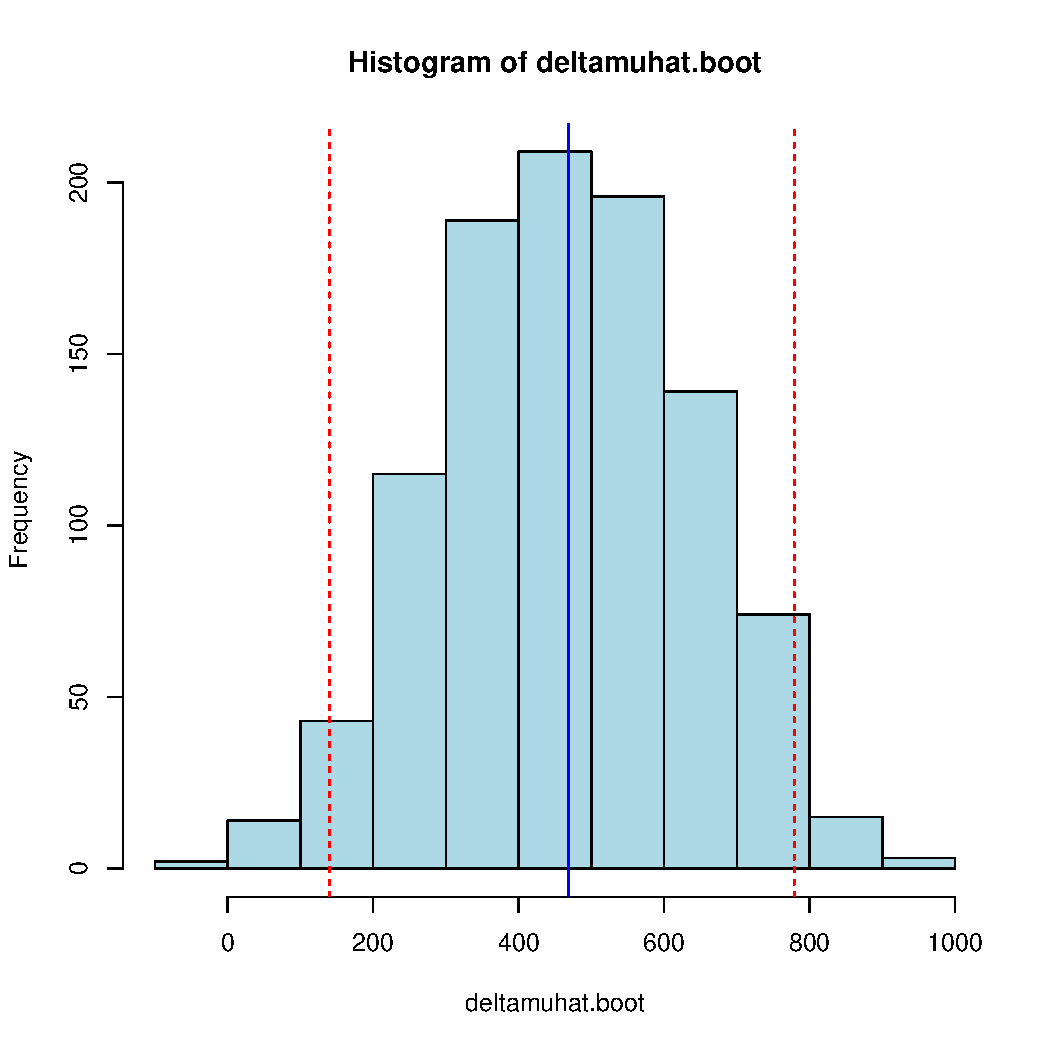
\includegraphics[width=\maxwidth]{figure/unnamed-chunk-9-1} 

}


\end{knitrout}
		\end{minipage}
	\end{figure}
	
	
\end{frame}


\begin{frame}[fragile,plain]
	%	\vspace*{-0.2in}
	\small
	\textbf{2.2 Bootstrap CI for mean difference using canned function (continued)}

		\begin{figure}
		\begin{minipage}[h]{0.45\linewidth}
\begin{knitrout}\tiny
\definecolor{shadecolor}{rgb}{0.969, 0.969, 0.969}\color{fgcolor}\begin{kframe}
\begin{alltt}
\hlkwd{summary}\hlstd{(betahat.boot)}
\end{alltt}
\begin{verbatim}
## 
## Number of bootstrap replications R = 999 
##             original bootBias bootSE bootMed
## (Intercept)  3365.59   2.7714 138.49 3365.49
## South         473.91  -7.8980 170.43  468.35
\end{verbatim}
\begin{alltt}
\hlkwd{confint}\hlstd{(betahat.boot)}
\end{alltt}
\begin{verbatim}
## Bootstrap bca confidence intervals
## 
##                 2.5 %    97.5 %
## (Intercept) 3086.0282 3634.6473
## South        144.5181  789.5421
\end{verbatim}
\end{kframe}
\end{knitrout}
			
		\end{minipage}
		\hspace{0.4cm}
		\begin{minipage}[h]{0.50\linewidth}
\begin{knitrout}\tiny
\definecolor{shadecolor}{rgb}{0.969, 0.969, 0.969}\color{fgcolor}

{\centering 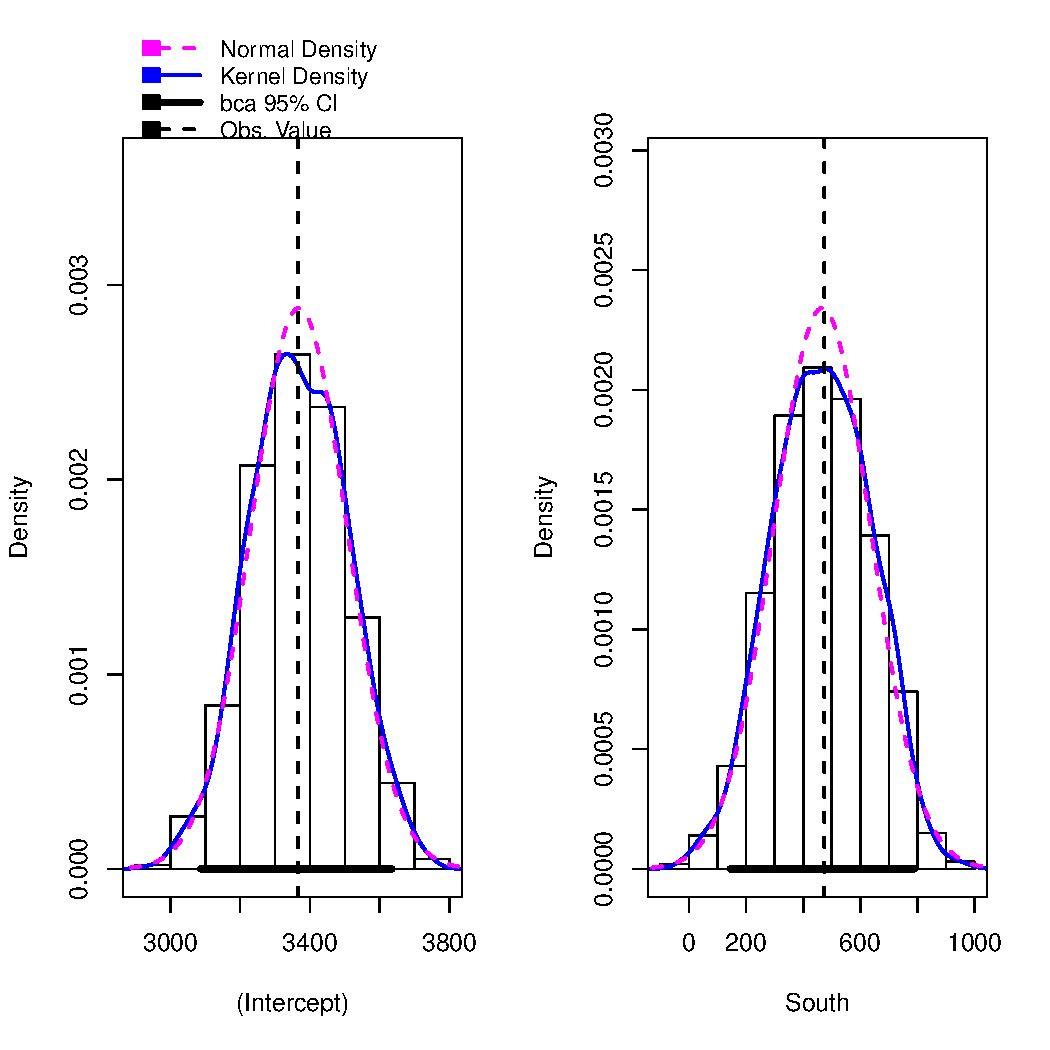
\includegraphics[width=\maxwidth]{figure/unnamed-chunk-11-1} 

}


\end{knitrout}
\end{minipage}
\end{figure}
	
	
\end{frame}




\begin{frame}[fragile,plain]
		\textbf{2.3 Bootstrap CI for mean difference using \texttt{boot} package}
\begin{figure}
	\begin{minipage}[h]{0.40\linewidth}
\begin{knitrout}\tiny
\definecolor{shadecolor}{rgb}{0.969, 0.969, 0.969}\color{fgcolor}\begin{kframe}
\begin{alltt}
\hlkwd{library}\hlstd{(boot)}
\hlcom{# function to obtain deltamu hat}
\hlstd{deltamu} \hlkwb{<-} \hlkwa{function}\hlstd{(}\hlkwc{data}\hlstd{,} \hlkwc{indices}\hlstd{) \{}
        \hlcom{# allows boot to select sample}
        \hlstd{d} \hlkwb{<-} \hlstd{data[indices,]}
        \hlstd{fit} \hlkwb{<-} \hlkwd{lm}\hlstd{(alt} \hlopt{~} \hlstd{South,} \hlkwc{data}\hlstd{=d)}
        \hlkwd{coef}\hlstd{(fit)[}\hlstr{"South"}\hlstd{]}
\hlstd{\}}

\hlstd{results} \hlkwb{<-} \hlstd{boot}\hlopt{::}\hlkwd{boot}\hlstd{(}\hlkwc{data} \hlstd{= depths,}
\hlkwc{statistic} \hlstd{= deltamu,} \hlkwc{R}\hlstd{=}\hlnum{999}\hlstd{)}

\hlkwd{boot.ci}\hlstd{(results)}
\end{alltt}
\begin{verbatim}
## BOOTSTRAP CONFIDENCE INTERVAL CALCULATIONS
## Based on 999 bootstrap replicates
## 
## CALL : 
## boot.ci(boot.out = results)
## 
## Intervals : 
## Level      Normal              Basic         
## 95%   (157.4, 800.6 )   (148.3, 798.3 )  
## 
## Level     Percentile            BCa          
## 95%   (149.5, 799.6 )   (158.4, 815.0 )  
## Calculations and Intervals on Original Scale
\end{verbatim}
\end{kframe}
\end{knitrout}
		
	\end{minipage}
	\hspace{0.4cm}
	\begin{minipage}[h]{0.50\linewidth}
\begin{knitrout}\tiny
\definecolor{shadecolor}{rgb}{0.969, 0.969, 0.969}\color{fgcolor}\begin{kframe}
\begin{alltt}
\hlkwd{plot}\hlstd{(results)}
\end{alltt}
\end{kframe}

{\centering 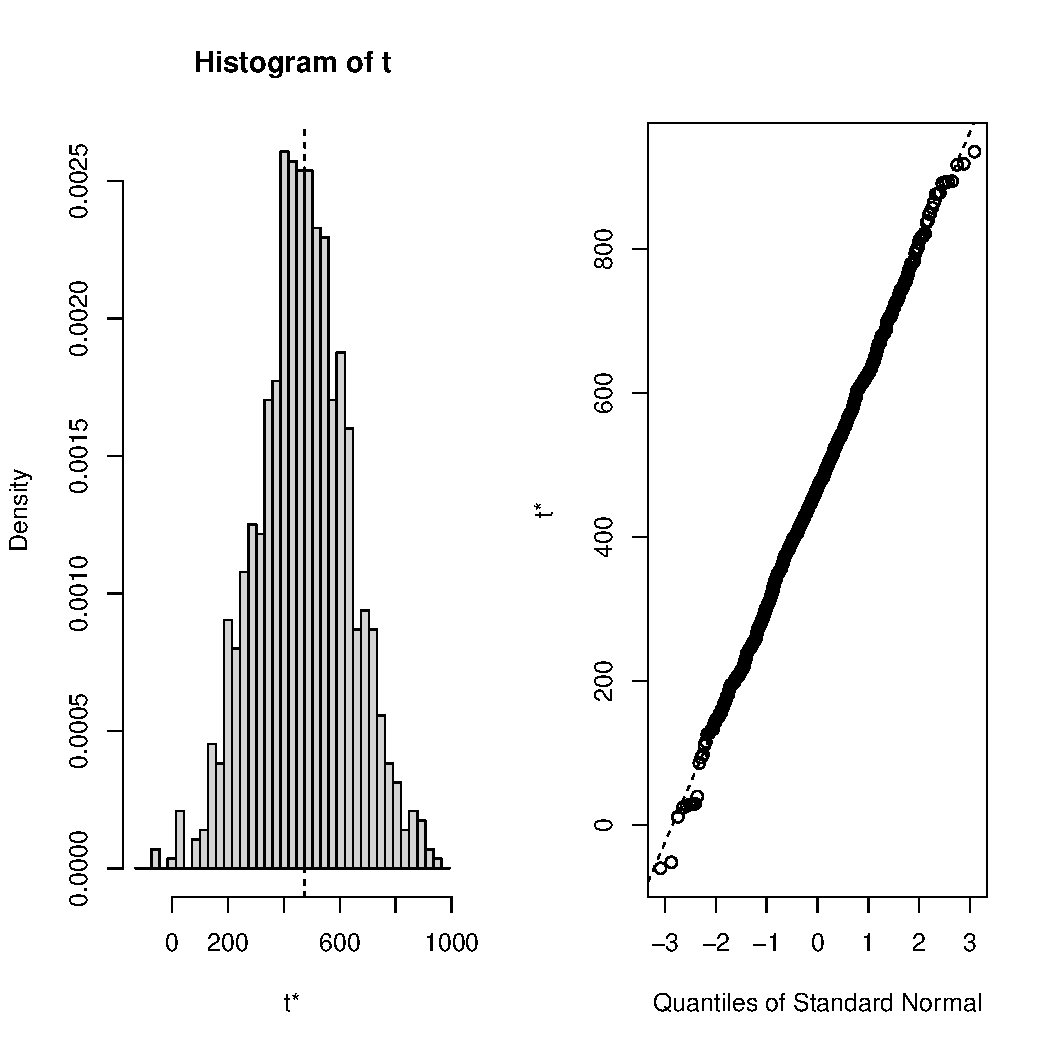
\includegraphics[width=\maxwidth]{figure/unnamed-chunk-13-1} 

}


\end{knitrout}
	\end{minipage}
\end{figure}
\end{frame}


\section{Permutation Testing}

\begin{frame}{Permutation Testing}
\begin{itemize}
	\item In testing a null hypothesis we need a test statistic that will have different values under the null hypothesis and the alternatives we	care about 
	\item We then need to compute the sampling distribution of the test	statistic when the null hypothesis is true. For some test statistics	and some null hypotheses this can be done analytically. 
	\item The pvalue is the probability that the test statistic would be at	least as extreme as we observed, if the null hypothesis is true.
	\item A permutation test gives a simple way to compute the sampling	distribution for any test statistic, under the null hypothesis that there is no effect (i.e. South is not a determinant of the mean depth of the ocean)
\end{itemize}
\end{frame}


\begin{frame}{Permutation Testing}
	\begin{itemize}
		\item To estimate the sampling distribution of the test statistic we
		need many samples generated under the strong null hypothesis.
		\item If the null hypothesis is true, changing the exposure would have
		no effect on the outcome. By randomly shuffling the determinants
		we can make up as many data sets as we like.
		\item If the null hypothesis is true, the shuffled data sets should look
		like the real data, otherwise they should look different from the real data.
		\item The ranking of the real test statistic among the shuffled test
		statistics gives a p-value
	\end{itemize}
\end{frame}




\begin{frame}[fragile]{Permutation Testing}
\begin{knitrout}\tiny
\definecolor{shadecolor}{rgb}{0.969, 0.969, 0.969}\color{fgcolor}\begin{kframe}
\begin{alltt}
\hlstd{one.test} \hlkwb{<-} \hlkwa{function}\hlstd{(}\hlkwc{x}\hlstd{,}\hlkwc{y}\hlstd{) \{}
   \hlstd{xstar} \hlkwb{<-} \hlkwd{sample}\hlstd{(x)}
   \hlkwd{mean}\hlstd{(y[xstar}\hlopt{==}\hlnum{1}\hlstd{])} \hlopt{-} \hlkwd{mean}\hlstd{(y[xstar}\hlopt{==}\hlnum{0}\hlstd{])}
\hlstd{\}}

\hlstd{null.dist} \hlkwb{<-} \hlkwd{replicate}\hlstd{(}\hlnum{1000}\hlstd{,} \hlkwd{one.test}\hlstd{(}\hlkwc{x} \hlstd{= depths}\hlopt{$}\hlstd{South,} \hlkwc{y} \hlstd{= depths}\hlopt{$}\hlstd{alt))}
\hlkwd{hist}\hlstd{(null.dist)}
\hlkwd{abline}\hlstd{(}\hlkwc{v}\hlstd{=}\hlkwd{coef}\hlstd{(fit)[}\hlstr{"South"}\hlstd{],} \hlkwc{lwd}\hlstd{=}\hlnum{2}\hlstd{,} \hlkwc{col}\hlstd{=}\hlstr{"blue"}\hlstd{)}
\end{alltt}
\end{kframe}

{\centering 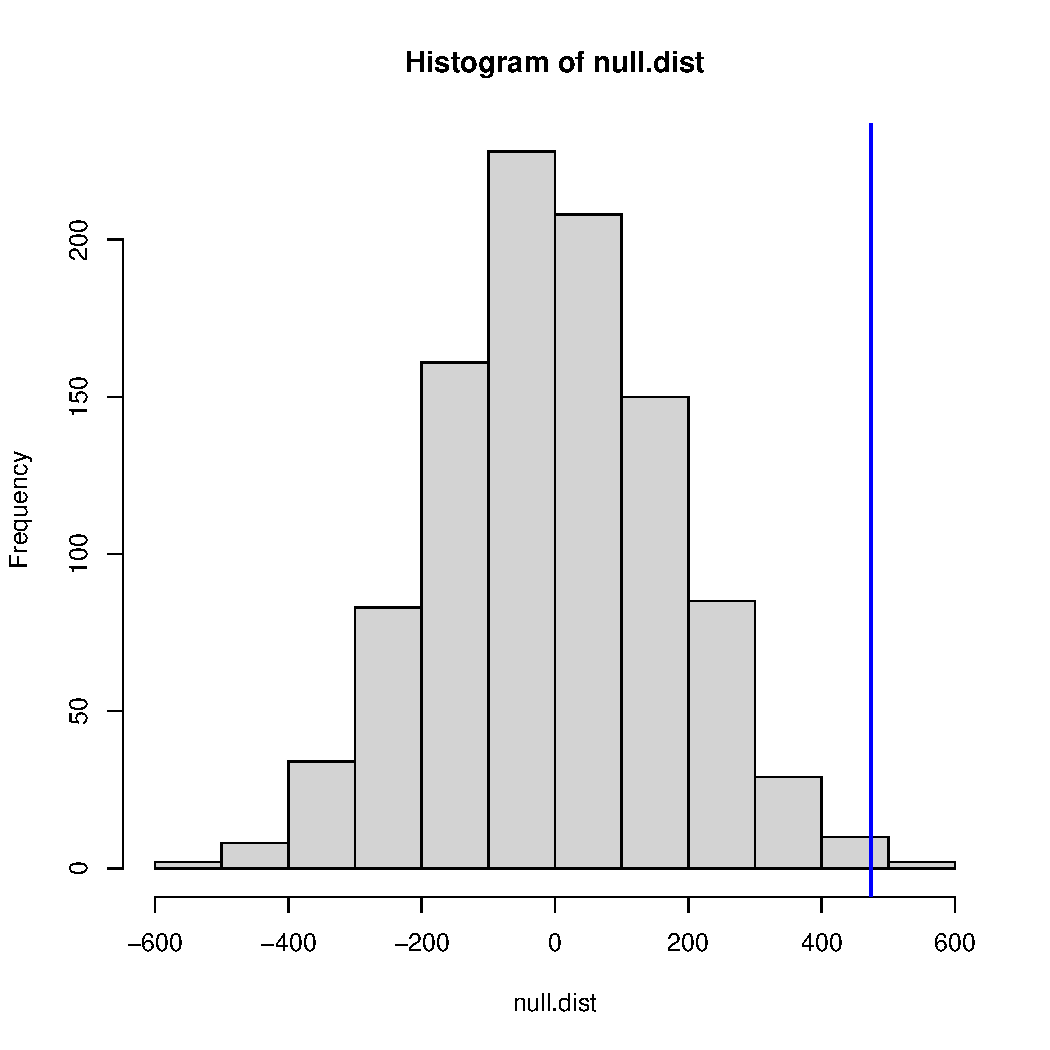
\includegraphics[width=0.5\textwidth]{figure/unnamed-chunk-14-1} 

}


\begin{kframe}\begin{alltt}
\hlkwd{mean}\hlstd{(}\hlkwd{abs}\hlstd{(null.dist)} \hlopt{>} \hlkwd{abs}\hlstd{(}\hlkwd{coef}\hlstd{(fit)[}\hlstr{"South"}\hlstd{]))}
\end{alltt}
\begin{verbatim}
## [1] 0.007
\end{verbatim}
\end{kframe}
\end{knitrout}
\end{frame}


\section{Ratio depth of ocean depths in north vs south hemisphere}

\begin{frame}[fragile,plain]
\vspace*{-1.1in}
\textbf{3. Ratio depth of ocean depths in north vs south hemisphere}
\begin{knitrout}\tiny
\definecolor{shadecolor}{rgb}{0.969, 0.969, 0.969}\color{fgcolor}\begin{kframe}
\begin{alltt}
\hlcom{# note: we are now using glm}
\hlstd{fit} \hlkwb{<-} \hlkwd{glm}\hlstd{(alt} \hlopt{~} \hlstd{South,} \hlkwc{data} \hlstd{= depths,} \hlkwc{family} \hlstd{=} \hlkwd{gaussian}\hlstd{(}\hlkwc{link}\hlstd{=log))}
\hlkwd{print}\hlstd{(}\hlkwd{summary}\hlstd{(fit),} \hlkwc{signif.stars} \hlstd{= F)}
\end{alltt}
\begin{verbatim}
## 
## Coefficients:
##             Estimate Std. Error t value Pr(>|t|)
## (Intercept)  8.12136    0.03603  225.41  < 2e-16
## South        0.13174    0.04791    2.75  0.00624
## 
## (Dispersion parameter for gaussian family taken to be 2940751)
## 
##     Null deviance: 1192876833  on 399  degrees of freedom
## Residual deviance: 1170417764  on 398  degrees of freedom
## AIC: 7096.8
## 
## Number of Fisher Scoring iterations: 5
\end{verbatim}
\end{kframe}
\end{knitrout}

\end{frame}


\begin{frame}[fragile,plain]
	\vspace*{-5.0in}
	\textbf{1. Mean depth of the ocean (continued)\footnotetext[1]{\tiny{this page is intentionally left blank}}}
	
\end{frame}


\begin{frame}[fragile]{Session Info}
	\tiny
	
\begin{knitrout}\tiny
\definecolor{shadecolor}{rgb}{0.969, 0.969, 0.969}\color{fgcolor}\begin{kframe}
\begin{verbatim}
R version 4.1.1 (2021-08-10)
Platform: x86_64-pc-linux-gnu (64-bit)
Running under: Pop!_OS 21.04

Matrix products: default
BLAS:   /usr/lib/x86_64-linux-gnu/openblas-pthread/libblas.so.3
LAPACK: /usr/lib/x86_64-linux-gnu/openblas-pthread/libopenblasp-r0.3.13.so

attached base packages:
[1] tools     stats     graphics  grDevices utils     datasets  methods  
[8] base     

other attached packages:
 [1] boot_1.3-27       car_3.0-9         carData_3.0-4     DT_0.16          
 [5] mosaic_1.7.0      Matrix_1.3-2      mosaicData_0.20.1 ggformula_0.9.4  
 [9] ggstance_0.3.4    lattice_0.20-41   kableExtra_1.2.1  socviz_1.2       
[13] gapminder_0.3.0   here_0.1          NCStats_0.4.7     FSA_0.8.30       
[17] forcats_0.5.1     stringr_1.4.0     dplyr_1.0.7       purrr_0.3.4      
[21] readr_1.4.0       tidyr_1.1.4       tibble_3.1.5      ggplot2_3.3.5    
[25] tidyverse_1.3.0   knitr_1.36       

loaded via a namespace (and not attached):
 [1] fs_1.5.0           lubridate_1.7.9    webshot_0.5.2      httr_1.4.2        
 [5] rprojroot_2.0.2    backports_1.2.1    utf8_1.2.2         R6_2.5.1          
 [9] DBI_1.1.1          colorspace_2.0-2   withr_2.4.2        tidyselect_1.1.1  
[13] gridExtra_2.3      leaflet_2.0.3      curl_4.3.2         compiler_4.1.1    
[17] cli_3.0.1          rvest_1.0.0        pacman_0.5.1       xml2_1.3.2        
[21] ggdendro_0.1.22    mosaicCore_0.8.0   scales_1.1.1       digest_0.6.28     
[25] foreign_0.8-81     rmarkdown_2.11.3   rio_0.5.16         pkgconfig_2.0.3   
[29] htmltools_0.5.2    highr_0.9          dbplyr_1.4.4       fastmap_1.1.0     
[33] htmlwidgets_1.5.3  rlang_0.4.12       readxl_1.3.1       rstudioapi_0.13   
[37] farver_2.1.0       generics_0.1.0     jsonlite_1.7.2     crosstalk_1.1.1   
[41] zip_2.2.0          magrittr_2.0.1     Rcpp_1.0.7         munsell_0.5.0     
[45] fansi_0.5.0        abind_1.4-5        lifecycle_1.0.1    stringi_1.7.5     
[49] MASS_7.3-53.1      plyr_1.8.6         grid_4.1.1         blob_1.2.1        
[53] ggrepel_0.8.2      crayon_1.4.1       cowplot_1.1.0      haven_2.3.1       
[57] splines_4.1.1      hms_1.1.1          pillar_1.6.4       reprex_0.3.0      
[61] glue_1.4.2         evaluate_0.14      data.table_1.14.2  modelr_0.1.8      
[65] vctrs_0.3.8        tweenr_1.0.1       cellranger_1.1.0   gtable_0.3.0      
[69] polyclip_1.10-0    assertthat_0.2.1   TeachingDemos_2.12 xfun_0.26         
[73] ggforce_0.3.2      openxlsx_4.1.5     broom_0.7.9        viridisLite_0.4.0 
[77] ellipsis_0.3.2    
\end{verbatim}
\end{kframe}
\end{knitrout}
	
\end{frame}





\end{document}
